\documentclass[russian,english]{llncs}
\usepackage[utf8]{inputenc}
\usepackage[T2A]{fontenc}
\usepackage[final]{graphicx}
\usepackage{epstopdf}
\usepackage[labelsep=period]{caption}
\usepackage[hyphens]{url}
\usepackage{amssymb,amsmath,mathrsfs}
\usepackage[russian,english]{babel}
%\usepackage{multicol}
\usepackage[ruled,vlined,linesnumbered,algo2e]{algorithm2e}
%\usepackage{algorithm}
%\usepackage[noend]{algorithmic}
\usepackage{color}
\usepackage{cmap}
\usepackage{array}
\usepackage{tikz}
\usepackage{pgfplots}
%\usepackage{verbatim}
\usepackage{standalone}
\usepackage{verbatim}
\usepackage{tikz}
\usetikzlibrary{patterns}

\tolerance=1000
\hbadness=5000
\newcommand{\const}{\mathrm{const}}
\newcommand{\tsum}{\mathop{\textstyle\sum}\limits}
\newcommand{\tprod}{\mathop{\textstyle\prod}\limits}
\newcommand{\cov}{\mathop{\rm cov}\limits}
\newcommand{\Dir}{\mathop{\rm Dir}\nolimits}
\newcommand{\norm}{\mathop{\rm norm}\limits}
\newcommand{\KL}{\mathop{\rm KL}\nolimits}
%\renewcommand{\geq}{\geqslant}
%\renewcommand{\leq}{\leqslant}
\newcommand{\eps}{\varepsilon}
\newcommand{\cond}{\mspace{3mu}{|}\mspace{3mu}}
\newcommand{\Loss}{\mathscr{L}}
\newcommand{\RR}{\mathbb{R}}
\newcommand{\cL}{\mathscr{L}}
\newcommand{\cP}{\mathscr{P}}
\newcommand{\kw}[1]{\textsf{#1}}
\SetKwFor{ForAll}{\textbf{for all}}{}{}

%... and these rows too.
\pgfplotsset{ every non boxed x axis/.append style={x axis line style=-},
     every non boxed y axis/.append style={y axis line style=-}}
\pgfplotsset{compat = 1.3}


\pagenumbering{gobble}
\newcounter{wavenum}

\setlength{\unitlength}{1cm}
% advance clock one cycle, not to be called directly
\newcommand*{\clki}{
  \draw (t_cur) -- ++(0,.0) -- ++(.5,0) -- ++(0,-.0) -- ++(.5,0) -- ++(0,.0)
    node[time] (t_cur) {};
}

\newcommand*{\MergerQueue}[3]{
  \fill[fill=#3]
                         (t_cur) -- ++( .0, .04) -- ++(#2-.0,0) -- ++(.0, -.04)
                         -- ++(-.0,-.04) -- ++(.0-#2,0) -- cycle;
  \path (t_cur) -- node[anchor=mid] {#1} ++(#2,0) node[time] (t_cur) {};
}

\newcommand*{\MQFull}[2][XXX]{
    \MergerQueue{#1}{#2}{red}
}

\newcommand*{\MQNormal}[2]{
    \MergerQueue{#1}{#2}{green}
}

\newcommand*{\bitvector}[6]{
  \fill[fill=#3, pattern=#5, pattern color=#4,fill opacity=#6]
                         (t_cur) -- ++( .0, .2) -- ++(#2-.0,0) -- ++(.0, -.18)
                         -- ++(-.0,-.18) -- ++(.0-#2,0) -- cycle;
  \path (t_cur) -- node[anchor=mid] {#1} ++(#2,0) node[time] (t_cur) {};
}

% \known{val}{length}
\newcommand*{\Wait}[2]{
    \bitvector{#1}{#2}{white}{white}{}{0.0}
}

% \unknown{length}
\newcommand*{\ProcBatchOne}[2][XXX]{
    \bitvector{#1}{#2}{orange}{orange}{}{1.0}
}

% \unknown{length}
\newcommand*{\ProcBatchTwo}[2][XXX]{
    \bitvector{#1}{#2}{yellow}{yellow}{}{1.0}
}

% \unknown{length}
\newcommand*{\Regularization}[2][XXX]{
    \bitvector{#1}{#2}{red}{red}{}{1.0}
}

% \unknown{length}
\newcommand*{\Normalization}[2][XXX]{
    \bitvector{#1}{#2}{green}{green}{}{1.0}
}

% \unknown{length}
\newcommand*{\Merge}[2][XXX]{
    \bitvector{#1}{#2}{blue}{blue}{}{1.0}
}

% \nextwave{name}
\newcommand{\nextwave}[1]{
  \path (0,\value{wavenum} * 0.5) node[left] {#1} node[time] (t_cur) {};
  \addtocounter{wavenum}{-1}
}

% \begin{wave}[clkname]{num_waves}{clock_cycles}
\newenvironment{wave}[3][\bf{time}]{
  \begin{tikzpicture}[draw=black, yscale=1.5,xscale=1.0]
    \tikzstyle{time}=[coordinate]
    \setlength{\unitlength}{1cm}
    \def\wavewidth{#3}
    \setcounter{wavenum}{0}
    \nextwave{#1}

    \draw[dotted] (t_cur) +(0,.1) node[above] {t=0\%} -- ++(0,2.8-#2);
    \clki
    \foreach \t in {1,...,\wavewidth}{
      \draw[dotted] (t_cur) +(0,.1) node[above] {\t0\%} -- ++(0,2.8-#2);
      \clki
    }
}{\end{tikzpicture}}

%%% End of timing.sty
\usepackage{verbatim}

\begin{document}
%%Analysis of Images, Social Networks, and Texts
\title{
    Parallel Non-blocking Deterministic Algorithm for Online Topic Modeling
}
\author{
    Oleksandr Frei\inst{1}
    \and
    Murat Apishev\inst{2}
}
\institute{\noindent
    Schlumberger Information Solutions,
    ~~\email{oleksandr.frei@gmail.com}
    \and
    Lomonosov Moscow State University,
    ~~\email{great-mel@yandex.ru}
}

\maketitle

\begin{abstract}
In this paper we present a new asynchronous algorithm for learning additively regularized topic models
and discuss the main architectural details of our implementation.
The key property of the new algorithm is that it behaves in a fully deterministic fashion,
which is typically hard to achieve in a non-blocking parallel implementation. The algorithm
%has been
had been
recently implemented in the BigARTM library (\texttt{http://bigartm.org}).
Our new algorithm is compatible with all features previously introduced in BigARTM library,
including multimodality, regularizers and scores calculation.
Previous BigARTM version was already faster than the alternative open source topic modeling packages such as Vowpal Wabbit or Gensim.
Yet, in our experiments we show that the new implementation spends even less time to achieve the same perplexity, has better CPU utilization and lower memory usage.

\vspace{1em}
\textbf{Keywords:}
    probabilistic topic modeling,
    Probabilistic Latent Sematic Analysis,
    Latent Dirichlet Allocation,
    Additive Regularization of Topic Models,
    stochastic matrix factorization,
    EM-algorithm,
    online learning,
    asynchronous and parallel computing,
    BigARTM.
\end{abstract}

\section{Introduction}

Deterministic behavior is an important property for any algorithm,
including those of a stochastic nature.
For the end users of a software system run-to-run reproducibility is a must-have property,
because this is what they expect based on their previous experience.
Indeed, refreshing a web-pages or re-doing an operation tend to
produce an identical result, regardless of how much software complexity is hidden behind the scenes.
For the researches determinism is also important
because it enables them to reproduce their old experiments
and study impact of various parameters on the result.
Finally, for the developers of the algorithm
determinism allow to reproduce bugs and write simple unit-tests with well-defined results.

Determinism is particularly hard to achieve
in concurrent implementations, because in a multi-threaded environment
it might not be sufficient to just fix a random seed or an initial approximation.
In this paper we present a deterministic modification of parallel non-blocking algorithm
for online topic modeling, previously developed for BigARTM library.
We implement new algorithm in BigARTM and demonstrate that new version converges faster
than previous algorithm in terms of perplexity,
yet being more efficient in CPU and memory usage.

The rest of the paper is organized as follows.
In~section~\ref{sec:Notation}
we introduce basic notation used throughout this paper.
In~sections~\ref{sec:Offline}, \ref{sec:Online}, \ref{sec:AsyncOnline}
we summarize Offline, Online and Asynchronous Online algorithms for learning ARTM models.
In~section~\ref{sec:Architecture}
we~compare the internal architecture of BigARTM library between versions v0.6 and v0.7.
In~section~\ref{sec:Experiments}
we~report results of our experiments on large datasets.
In~section~\ref{sec:Conclusions}
we~discuss advantages, limitations and open problems of BigARTM.

%sashafrey:
%really technical topics in my opinion does not belong to AISTconf article;
%it would be more appropriate to discuss the following in the full 12-page article in http://www.ispras.ru/en/ journal
%\begin{itemize}
%    \item Details of CLI interface and python interface, usage examples
%    \item List new features: coherence score and regularizer, classification, documents markdown (aka $p_{tdw}$ matrices)
%    \item Our technologies (Protobuf for low-level C API, Boost Serialize for import/export, GLog, GFlags, GTest, etc)
%    \item Our build solution and CI solution (CMake, Visual Studio, GitHub, Git submodules, Travis, Apveyour, Read-The-Docs)
%    \item Why people care about run-to-run reproducibility
%    https://software.intel.com/en-us/articles/consistency-of-floating-point-results-using-the-intel-compiler
%\end{itemize}

\section{Notation}
\label{sec:Notation}

Let
$D$ denote a finite set (collection) of texts and
$W$ denote a~finite set (vocabulary) of all terms from these texts.
Let
$n_{dw}$ denote the number of occurrences of a term $w \in W$ in a document $d \in D$;
$n_{dw}$ values form a sparse matrix of size $|W| \times |D|$,
known as \emph{bag-of-words} representation of the collection.

Given an $(n_{dw})$ matrix, an additively-regularized topic model (ARTM) finds two matrices:
$\Phi = \{\phi_{wt}\}$ and $\Theta = \{\theta_{td}\}$,
of sizes $|W| \times |T|$ and $|T| \times |D|$ respectively,
where $|T|$ is a used-defined number of \emph{topics} in the model.
Matrices $\Phi$ and $\Theta$
provide a compressed representation of the $(n_{dw})$ matrix:
\[
n_{dw} \approx n_d \sum_{t \in T} \phi_{wt} \theta_{td}, \text { for all } d \in D, w \in W,
\]
where $n_d = \sum_{w \in W} n_{dw}$ denotes the total number of terms in a document $d$.
%Matrices $\Phi$ and $\Theta$ are \emph{stochastic}, e.g. their elements are non-negative and all columns are normalized to unity.
%In the sequel we will use ``norm'' operator to transform
%a~real vector into a discrete distribution.
%For example some arbitrary positive values $n_{td}$ and $n_{wt}$
%can be turned into $\theta_{td}$ and $\phi_{wt}$ as follows:
%\begin{align}
%    \theta_{td} = \norm_{t\in T} n_{td} = n_{td} \big/ \sum_{s\in T} n_{sd}; \\
%    \phi_{wt} = \norm_{w \in W} n_{wt} = n_{wt} \big/ \sum_{v \in W} n_{vt}.
%\end{align}

To learn $\Phi$ and $\Theta$ from $(n_{dw})$ ARTM maximizes
the log-likelihood, regularized via an additional penalty term $R(\Phi, \Theta)$:
\begin{gather}
\label{eq:ARTM}
    \sum_{d\in D}\sum_{w\in W} n_{dw} \ln \sum_{t\in T} \phi_{wt} \theta_{td} + R(\Phi, \Theta)
    \;\to\; \max_{\Phi,\Theta}.
\end{gather}
With no regularization (${R=0}$) it corresponds to PLSA~\cite{hofmann99plsi}.
Many Bayesian topic models can be considered
as special cases of ARTM with different regularizers~$R$,
as shown in~\cite{voron14mlj,voron14aist}.

In \cite{voron14dan-eng} it is shown that the \mbox{local} maximum $(\Phi,\Theta)$
of the problem~\eqref{eq:ARTM} satisfies
\begin{align}
    \label{eq:Estep}
    p_{tdw} &= \norm_{t\in T} \bigl(\phi_{wt}\theta_{td}\bigr);
\\
    \label{eq:Mstep:phi}
    \phi_{wt} &= \norm_{w\in W}
        \biggl(
            \sum_{d\in D} n_{dw} p_{tdw} + \phi_{wt} \frac{\partial R}{\partial \phi_{wt}}
        \biggr);
%    \phi_{wt} &= \norm_{w\in W}
%        \biggl(
%            n_{wt} + r_{wt}
%        \biggr);
%    \quad
%    n_{wt} = \sum_{d\in D} n_{dw} p_{tdw};
%    \quad
%    r_{wt} = \phi_{wt} \frac{\partial R}{\partial \phi_{wt}};
\\
    \label{eq:Mstep:theta}
    \theta_{td} &= \norm_{t\in T}
        \biggl(
            \sum_{w\in d} n_{dw} p_{tdw} + \theta_{td} \frac{\partial R}{\partial \theta_{td}}
        \biggr);
%    \theta_{td} &= \norm_{t\in T}
%        \biggl(
%            n_{td} + r_{td}
%        \biggr);
%    \quad
%    n_{td} = \sum_{w\in d} n_{dw} p_{tdw};
%    \quad
%    r_{td} = \theta_{td} \frac{\partial R}{\partial \theta_{td}};
        %\sum_{m=1}^M \tau_m \!\!\sum_{w\in W^m}\!\!\! n_{dw} p_{tdw};
\end{align}
where operator
$\norm_{i \in I} x_i = \frac{\max\{x_i,0\}}{\sum\limits_{j\in I} \max\{x_j,0\}}$
transforms a~vector $(x_i)_{i \in I}$ to a~discrete distribution.

Learning of $\Phi$ and $\Theta$ from \eqref{eq:Estep}--\eqref{eq:Mstep:theta} can be done by EM-algorithm,
which starts from a random initial approximation and iterates
E-step \eqref{eq:Estep} and
M-steps \eqref{eq:Mstep:phi},\eqref{eq:Mstep:theta}
until convergence.
In the sequel we discuss several variations of such EM-algorithm,
which are all based on the above formulas but differ in the way how operations are ordered and grouped together.

%In additional to plain text many collections has additional data,
%such as authors, class or category labels, date-time stamps.
%In \cite{vfardy15cikmtm} this data can be represented as \emph{modalities},
%where the overall vocabulary $W$ is split into $M$ subsets
%$W = W^1 \sqcup \dots \sqcup W^M$, one subset per modality,
%and $\Phi$ matrix is normalized independently within each modality:
%\begin{align}
%    \sum_{w \in W^m} \phi_{wt} = 1, \; \text{ for all } t \in T, m = 1, \dots, M \\\notag
%\end{align}


\section{Offline algorithm}
\label{sec:Offline}

\SetAlgoSkip{}
\begin{algorithm2e}[t]
\caption{Offline algorithm}
\label{alg:Offline}
\BlankLine
\KwIn{collection $D$;}
\KwOut{matrix $\Phi = (\phi_{wt})$;}
\BlankLine
initialize $(\phi_{wt})$\;
form batches $D := D_1 \sqcup D_2 \sqcup \dots \sqcup D_B$\;
\Repeat{$(\phi_{wt})$ converges}{
    %$\tilde n_{wt} := 0$ for all $w \in W$ and $t \in T$\;
    %\ForAll{documents $d \in D$} {
    %    $(\tilde n_{wt}) := (\tilde n_{wt}) + \kw{ProcessDocument}(d, \Phi)$\;
    %}
    $(n_{wt}) := \mathlarger\sum\limits_{b=1, \dots, B} \; \mathlarger\sum\limits_{d \in D_b} \; \kw{ProcessDocument}(d, \Phi)$\;
    $(\phi_{wt}) := \norm_{w \in W} (n_{wt} + \phi_{wt} \frac{\partial R}{\partial \phi_{wt}})$\;
}
\end{algorithm2e}
\begin{algorithm2e}[t]
\caption{\kw{ProcessDocument}($d, \Phi$)}
\label{alg:ProcessDocument}
\BlankLine
\KwIn{document $d \in D$, matrix $\Phi=(\phi_{wt})$;}
\KwOut{matrix $(\tilde n_{wt})$;}
\BlankLine
initialize $\theta_{td} := \frac{1}{|T|}$ for all $t \in T$\;
\Repeat{$\theta_d$ converges}{
    $p_{tdw} := \norm_{t\in T} \bigl(\phi_{wt}\theta_{td}\bigr)$ for all $w\in d$ and $t \in T$\;
    $\theta_{td} := \norm_{t\in T}
        \bigl(
            \sum_{w\in d} n_{dw} p_{tdw} + \theta_{td} \frac{\partial R}{\partial \theta_{td}}
        \bigr)$ for all $t \in T$\;
}
$\tilde n_{wt} := n_{dw} p_{tdw}$ for all $w \in d$ and $t \in T$\;
\end{algorithm2e}

%\begin{figure}
%\centering
%\begin{wave}{6}{10}
%\nextwave{15864} \Wait{ }{9.45095925655}\Normalization[ ]{0.549040743454}
%\nextwave{16916} \Wait{ }{0.117635895262}\ProcBatchOne[ ]{2.19608818345} \Wait{ }{0.117635895262} \ProcBatchOne[ ]{1.41181771905} \Wait{ }{0.117593825681} \ProcBatchOne[ ]{1.56862506795} \Wait{ }{0.117715360024} \ProcBatchOne[ ]{1.72546981204} \Wait{ }{0.117635895262} \ProcBatchOne[ ]{1.8431057073}
%\nextwave{14388} \Wait{ }{0.156886813664}\ProcBatchOne[ ]{2.31368200913} \Wait{ }{0.117677964842} \ProcBatchOne[ ]{0.588212197093} \Wait{ }{0.0784644416221} \ProcBatchOne[ ]{0.980370801281} \Wait{ }{0.117673290444} \ProcBatchOne[ ]{1.68626096322} \Wait{ }{0.117673290444} \ProcBatchOne[ ]{0.901906359658} \Wait{ }{0.117635895262} \ProcBatchOne[ ]{1.64712690476}
%\nextwave{18080} \Wait{ }{0.0}\ProcBatchOne[ ]{1.05887263809} \Wait{ }{0.117635895262} \ProcBatchOne[ ]{1.60779652159} \Wait{ }{0.0784223720419} \ProcBatchOne[ ]{0.901985824421} \Wait{ }{0.117635895262} \ProcBatchOne[ ]{0.901948429239} \Wait{ }{0.0784597672243} \ProcBatchOne[ ]{0.43140952259} \Wait{ }{0.0783849768594} \ProcBatchOne[ ]{0.941157278061} \Wait{ }{0.117673290444} \ProcBatchOne[ ]{1.72546981204}
%\nextwave{10108} \Wait{ }{0.117635895262}\ProcBatchOne[ ]{2.11766581141} \Wait{ }{0.156886813664} \ProcBatchOne[ ]{1.72546981204} \Wait{ }{0.117635895262} \ProcBatchOne[ ]{1.6862983584} \Wait{ }{0.156844744084} \ProcBatchOne[ ]{1.88231923052}
%\end{wave}
%\caption{Gantt chart for Offline algorithm} \label{fig:gantt:offline}
%\end{figure}

The offline algorithm is given by
Fig. \ref{alg:Offline} (\kw{Offline algorithm}) and
Fig. \ref{alg:ProcessDocument} (\kw{ProcessDocument}).


Fig. \ref{fig:gantt:offline} illustrates how it works.
Orange boxes correspond to the time spent in processing an individual batch.
Green box correspond to the time spent to normalize $n_{wt}$ values and produce a new $p_{wt}$ matrix.

Key step of the algorithm is $\kw{ProcessDocument}$ subroutine
that generates a matrix $\hat n_{wt}$ of size $n_d \times |T|$.
These values describe contribution of the tokens from the document into the final $\Phi$ matrix.
Then the offline algorithm aggregates $\hat n_{wt}$ values across all documents in the collection.
After normalization they form a new $\Phi$ matrix for the next iteration.
Note that $\theta_{td}$ values appear only within $\kw{ProcessDocument}$ subroutine.
This makes the algorithm efficient in its memory usage,
allowing implementation to not store the entire theta matrix at any given time.
Instead, $\theta_{td}$ values are recalculated from scratch on every pass through the collection.

\section{Online}

Online EM-Algorithm is given by Fig. \ref{alg:Online}.
Fig. \ref{fig:gantt:online} illustrates how it works.
Orange and yellow boxes correspond to the time spent in processing an individual batch.
The color indicate which version of the $p^i_{wt}$ matrix was used to process each batch
(orange for even $i$, yellow for odd $i$).
Blue box correspond to the time spend in merging $n_{wt}$ with $\hat n_wt$,
Green box is, as before, the time spent to normalize $n_{wt}$ values and produce a new $p_{wt}$ matrix.

To improve convergence rate of the algorithm
the collection is split into ``batches'',
$D := D_1 \sqcup D_2 \sqcup \dots \sqcup D_B$,
and the algorithm is adjusted so that
matrix $\Phi$
is re-calculated after every $\eta$ batches.
This leads to more frequent updates of $\Phi$ matrix, which are performed as the algorithm scans through the collection.
To simplify the notation
we introduce a trivial subroutine
\[
\kw{ProcessBatches}(\{D_b\}, \Phi) = \mathlarger\sum\limits_{D_b} \mathlarger\sum\limits_{d \in D_b} \; \kw{ProcessDocument}(d, \Phi) \\
\]
that aggregates the output of $\kw{ProcessDocument}$ across specific batches at a constant $\Phi$ matrix.
The algorithm is then given by listing \ref{alg:Online}.

Key difference is that the cumulative sum $n_{wt}$ is discounted by a factor $\rho_i < 1$,
which depends on the iteration. Typical strategy is to use $\rho_i = (\tau_0 + i)^{-\kappa}$,
where typical values for $\tau_0$ are between $64$ and $1024$, for $\kappa$ --- between $0.5$ and $0.7$.

\SetAlgoSkip{}
\begin{algorithm2e}[h]
\caption{Online algorithm} %\mbox{regularized} topic modeling
\label{alg:Online}
\BlankLine
\KwIn{collection $D$, parameters $\eta, \tau_0, \kappa$;}
\KwOut{matrix $\Phi = (\phi_{wt})$;}
\BlankLine
form batches $D := D_1 \sqcup D_2 \sqcup \dots \sqcup D_B$\;
initialize $(\phi^0_{wt})$\;
\ForAll{update $i = 1, \dots, \lfloor B / \eta \rfloor$} {
    $(\hat n^i_{wt}) := \kw{ProcessBatches}(\{D_{\eta (i - 1) + 1}, \dots, D_{\eta i}\}, \Phi^{i - 1})$\;
    $\rho_i := (\tau_0 + i)^{-\kappa}$\;
    $(n^{i}_{wt}) := \rho_i \cdot (n^{i-1}_{wt}) + (1 - \rho_i) \cdot (\hat n^{i}_{wt})$\;
    $(\phi^{i}_{wt}) := \norm_{w \in W} (n^{i}_{wt} + \phi^{i - 1}_{wt} \frac{\partial R}{\partial \phi_{wt}})$\;
}
\end{algorithm2e}

%\begin{figure}
%\centering
%\begin{wave}{6}{10}
%\nextwave{23752} \Wait{ }{0.0332919679409}\ProcBatchTwo[ ]{0.732105963895} \Wait{ }{0.865238135943} \ProcBatchOne[ ]{0.249592576998} \Wait{ }{1.58067431606} \ProcBatchTwo[ ]{0.831946168002} \Wait{ }{1.61398215054} \ProcBatchOne[ ]{0.532441422221} \Wait{ }{1.49750587905} \ProcBatchTwo[ ]{0.748759881136}
%\nextwave{4448} \Wait{ }{0.0332919679409}\ProcBatchTwo[ ]{0.798654200062} \Wait{ }{0.81531010062} \ProcBatchOne[ ]{0.399344949889} \Wait{ }{1.41430174232} \ProcBatchTwo[ ]{0.665555744411} \Wait{ }{0.0665502194838} \ProcBatchTwo[ ]{0.881892053184} \Wait{ }{0.831930301462} \ProcBatchOne[ ]{0.831946168002}
%\nextwave{21464} \Wait{ }{0.898512254026}\Merge[ ]{0.366070831805} \Wait{ }{0.0332562682254} \Normalization[ ]{0.183044340832} \Wait{ }{1.21462133411} \Merge[ ]{0.366086698346} \Wait{ }{0.0332562682254} \Normalization[ ]{0.166390423591} \Wait{ }{1.86357472754} \Merge[ ]{0.366052981948} \Wait{ }{0.033258251543} \Normalization[ ]{0.183042357514} \Wait{ }{1.28118742013} \Merge[ ]{0.482529253438} \Wait{ }{0.0499121687835} \Normalization[ ]{0.199680408214} \Wait{ }{1.38102762424} \Merge[ ]{0.665557727729} \Wait{ }{0.0332741180832} \Normalization[ ]{0.199664541674}
%\nextwave{16912} \Wait{ }{0.0332919679409}\ProcBatchTwo[ ]{0.715485763053} \Wait{ }{0.881858336786} \ProcBatchOne[ ]{0.199646691816} \Wait{ }{0.0499458851814} \ProcBatchOne[ ]{0.765364215438} \Wait{ }{0.798672049919} \ProcBatchTwo[ ]{1.01499050883} \Wait{ }{1.39766369162} \ProcBatchOne[ ]{0.366052981948} \Wait{ }{0.0332919679409} \ProcBatchOne[ ]{0.698813995954} \Wait{ }{0.998354441451} \ProcBatchTwo[ ]{1.09815894584}
%\nextwave{22756} \Wait{ }{0.0}\ProcBatchTwo[ ]{0.449272985212} \Wait{ }{0.033258251543} \ProcBatchTwo[ ]{0.382706899188} \Wait{ }{0.798656183379} \ProcBatchOne[ ]{0.698831845812} \Wait{ }{1.0981767957} \ProcBatchTwo[ ]{0.898512254026} \Wait{ }{1.54741606451} \ProcBatchOne[ ]{0.865238135943}
%\end{wave}
%\caption{Gantt chart for new online algorithm} \label{fig:gantt:online}
%\end{figure}

A reasonable approach to speedup the online algorithm is to introduce concurrency in the $\kw{ProcessBatches}$ subroutine.
Indeed, multiple threads can simply process batches $D_{\eta (i - 1) + 1}, \dots, D_{\eta i}$ in parallel,
given that they synchronize writes $\hat n_{wt}$ values into the resulting matrix.
The problem with this approach is that all threads will have no useful work to do during steps $5$, $6$ and $7$ of the algorithm.
The threads can not start processing the next batches because a new version of $\Phi$ matrix is not ready yet.
In the next section we present a simple modification of the online algorithm that turns it into an asynchronous non-blocking algorithm.

\section{Asynchronous online algorithm}
\label{sec:AsyncOnline}

Asynchronous online EM-Algorithm is given by Fig. \ref{alg:AsyncOnline}.
Fig. \ref{fig:gantt:AsyncOnline} illustrates how it works.
The color scheme for the boxes is as in Fig. \ref{fig:gantt:AsyncOnline}.

\SetAlgoSkip{}
\begin{algorithm2e}[h]
\caption{Asynchronous online algorithm} %\mbox{regularized} topic modeling
\label{alg:AsyncOnline}
\BlankLine
\KwIn{collection $D$, parameters $\eta, \tau_0, \kappa$;}
\KwOut{matrix $\Phi = (\phi_{wt})$;}
\BlankLine
form batches $D := D_1 \sqcup D_2 \sqcup \dots \sqcup D_B$\;
initialize $(\phi^0_{wt})$\;
$(\hat n^1_{wt}) := \kw{AsyncProcessBatches}(\{D_{1}, \dots, D_{\eta}\}, \Phi^0)$\;
\ForAll{update $i = 1, \dots, \lfloor B / \eta \rfloor - 1$} {
    $(\hat n^{i+1}_{wt}) := \kw{AsyncProcessBatches}(\{D_{\eta i + 1}, \dots, D_{\eta i + \eta}\}, \Phi^{i-1})$\;
    $\kw{Await}(\hat n^i_{wt})$\;
    $\rho_i := (\tau_0 + i)^{-\kappa}$\;
    $(n^{i}_{wt}) := \rho_i \cdot (n^{i-1}_{wt}) + (1 - \rho_i) \cdot (\hat n^{i}_{wt})$\;
    $(\phi^{i}_{wt}) := \norm_{w \in W} (n^{i}_{wt} + \phi^{i-1}_{wt} \frac{\partial R}{\partial \phi_{wt}})$\;
}
\end{algorithm2e}

%\begin{figure}
%\centering
%\begin{wave}{6}{10}
%\nextwave{23796} \Wait{ }{0.0}\ProcBatchTwo[ ]{0.804602386207} \Wait{ }{0.0574647485947} \ProcBatchTwo[ ]{0.689672889017} \Wait{ }{0.0287306616923} \ProcBatchOne[ ]{0.373556830571} \Wait{ }{1.83909459368} \ProcBatchTwo[ ]{1.32182280087} \Wait{ }{0.0861988354971} \ProcBatchOne[ ]{1.35058086424}
%\nextwave{24032} \Wait{ }{1.89659016917}\Merge[ ]{0.919504481716} \Wait{ }{0.258623908171} \Normalization[ ]{0.402287492263} \Wait{ }{0.229889821269} \Merge[ ]{0.775871724514} \Wait{ }{0.0287306616923} \Normalization[ ]{0.344822743669} \Wait{ }{1.17815921678} \Merge[ ]{0.71840355071} \Wait{ }{0.0574647485947} \Normalization[ ]{0.287357995074} \Wait{ }{0.804602386207} \Merge[ ]{0.660938802115} \Wait{ }{0.0287032600121} \Normalization[ ]{0.287357995074} \Wait{ }{0.0574647485947} \Merge[ ]{0.660938802115} \Wait{ }{0.0574647485947} \Normalization[ ]{0.344822743669}
%\nextwave{17464} \Wait{ }{0.11498772576}\ProcBatchTwo[ ]{1.58041588215} \Wait{ }{0.0862262371773} \ProcBatchOne[ ]{1.29308871397} \Wait{ }{0.689672889017} \ProcBatchTwo[ ]{0.775840897624} \Wait{ }{0.0861988354971} \ProcBatchTwo[ ]{1.35061169113} \Wait{ }{0.0574373469145} \ProcBatchOne[ ]{0.488513729441} \Wait{ }{0.919531883396} \ProcBatchTwo[ ]{1.29314694254}
%\nextwave{12172} \Wait{ }{0.11498772576}\ProcBatchTwo[ ]{1.72410686792} \Wait{ }{0.0861988354971} \ProcBatchOne[ ]{1.63793885932} \Wait{ }{0.258623908171} \ProcBatchTwo[ ]{1.43681052663} \Wait{ }{0.0861680086069} \ProcBatchOne[ ]{1.23562396537} \Wait{ }{0.862067134802} \ProcBatchTwo[ ]{1.32185020255}
%\nextwave{10536} \Wait{ }{0.0574921502749}\ProcBatchTwo[ ]{1.0631988927} \Wait{ }{0.0862262371773} \ProcBatchOne[ ]{0.689672889017} \Wait{ }{0.0861988354971} \ProcBatchOne[ ]{1.14942512988} \Wait{ }{0.632177313532} \ProcBatchTwo[ ]{0.804602386207} \Wait{ }{0.60341582495} \ProcBatchOne[ ]{1.14942512988} \Wait{ }{0.11496032408} \ProcBatchOne[ ]{1.40807643973}
%\end{wave}
%\caption{Gantt chart for async online algorithm} \label{fig:gantt:AsyncOnline}
%\end{figure}

Adding delay and grouping several batches into a batchset negatively impact convergence,
but let utilize full CPU capacity of the machine.
In the experiments we demonstrate that on large datasets the resulting algorithm
is able to achieve better performance quicker that non-parallel or synchronous algorithm.

\section{New architecture}
\label{sec:Architecture}

Fig. \ref{fig:diagramm_artm_core} illustrates old architecture of BigARTM used up to version 0.6.
Fig. \ref{fig:gantt:oldonline} illustrates how the old architecture was used to implement a non-deterministic online algorithm.
Fig. \ref{fig:diagramm_artm_core_v07} illustrates new architecture of BigARTM used starting from version 0.7.


TBD: explain how \ref{Online} is parallelized in the previous BigARTM version.
Explain why it was non-deterministic.
Explain that non-deterministic version has negative impact on convergence.

In the new architecture we removed DataLoader thread,
which previously was responsible for loading batches from disk.
In the new architecture data loading happens directly from each processor thread.
This simplified the architecture without any lose in performance.

We also removed Merger thread, which previously was responsible
for merging $\hat n_{wt}$ --- model increments, produced on individual batches.
In a new architecture all increments are added to the final $\hat n_{wt}$ matrix
concurrently from processor threads.
To synchronize write access to this data structure we require that
no threads simultaneously update the same row in $\hat n_{wt}$ matrix.
Thus, the data for distinct words could be updated in parallel.
To enforce this behaviour we create one spin lock, $l_w$, for each word in global dictionary $W$.
After processing a batch the processor threads loops through local batch dictionary,
and for each $w \in W_b$ acquire the corresponding lock $l_w$.
%ToDo: measure collision ratio.
His approach of aggregating results across threads is taken from \cite{smola10architecture},
where the same pattern was used to update a shared stated in distributed topic modeling architecture.
In our case the same idea is applied to aggregating data in shared memory.

\begin{figure}[t]
\begin{centering}
%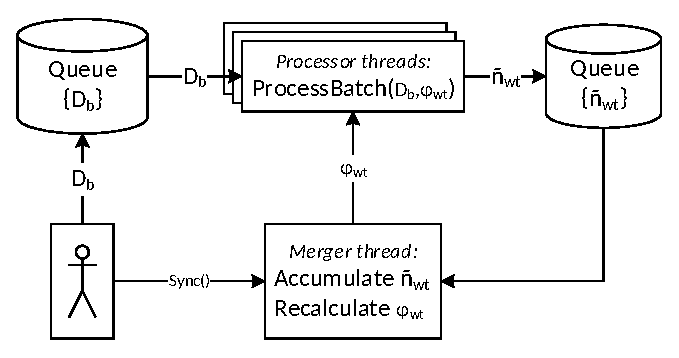
\includegraphics[height=39mm]{diagramm_artm_core.eps}
\caption{Diagram of parallelization components}
\label{fig:diagramm_artm_core}
\end{centering}
\end{figure}

\begin{figure}[t]
\begin{centering}
%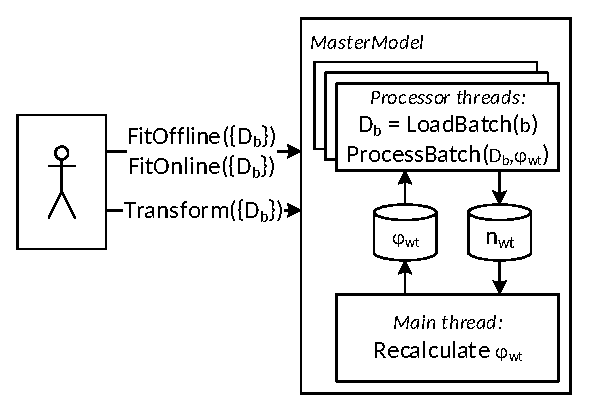
\includegraphics[height=54mm]{diagramm_artm_core_v07.eps}
\caption{Diagram of parallelization components (new architecture)}
\label{fig:diagramm_artm_core_v07}
\end{centering}
\end{figure}

%\begin{figure}
%\centering
%\begin{wave}{6}{10}
%\nextwave{10596} \Wait{ }{0.122939567821}\ProcBatchTwo[ ]{1.96726757211} \Wait{ }{0.122895601513} \ProcBatchTwo[ ]{1.88526552231} \Wait{ }{0.122939567821} \ProcBatchOne[ ]{1.80334651997} \Wait{ }{0.0819190023361} \ProcBatchOne[ ]{1.02457130407} \Wait{ }{0.122978648984} \ProcBatchTwo[ ]{1.721305389}
%\nextwave{17976} \Wait{ }{0.0409814843221}\ProcBatchTwo[ ]{1.02465435154} \Wait{ }{0.0819190023361} \ProcBatchTwo[ ]{1.27048952087} \Wait{ }{0.122934682676} \ProcBatchTwo[ ]{1.88526552231} \Wait{ }{0.082002049807} \ProcBatchOne[ ]{1.06554790325} \Wait{ }{0.0819629686442} \ProcBatchOne[ ]{1.55738433686} \Wait{ }{0.0409814843221} \ProcBatchTwo[ ]{0.532817917932} \Wait{ }{0.0819141171907} \ProcBatchTwo[ ]{0.655757485752}
%\nextwave{15212} \Wait{ }{0.082002049807}\ProcBatchTwo[ ]{1.84424495682} \Wait{ }{0.122939567821} \ProcBatchTwo[ ]{1.8032634725} \Wait{ }{0.123022615292} \ProcBatchOne[ ]{2.09011920732} \Wait{ }{0.082002049807} \ProcBatchOne[ ]{1.6393473055} \Wait{ }{0.286855734819} \ProcBatchTwo[ ]{1.92620304032}
%\nextwave{16956} \Wait{ }{0.0}\ProcBatchTwo[ ]{0.573799402254} \Wait{ }{0.0819580834989} \ProcBatchTwo[ ]{2.45902095825} \Wait{ }{0.122978648984} \ProcBatchTwo[ ]{1.84420099051} \Wait{ }{0.409839268948} \ProcBatchOne[ ]{2.04922565561} \Wait{ }{0.0819580834989} \ProcBatchTwo[ ]{1.02457130407}
%\end{wave}
%\caption{Gantt chart for old online algorithm (TBD: include merger thread here)} \label{fig:gantt:oldonline}
%\end{figure}

\section{Experiments}
\label{sec:Experiments}

Fig. \ref{fig:compare16}, \ref{fig:compare12} compare the perplexity as a function of time spend by four algorithms ---
offline,
online,
asynchronous Online,
and old non-deterministic implementation of the online algorithm.
Each point in the figure corresponds to a moment when the library finished a complete scan of the collection.
Each algorithm was given a fixed budget (30 minutes in the first chart, 40 minutes in the second chart).
Lower perplexity means better result.

%\begin{figure}
%\centering
%\begin{tikzpicture}
%    \begin{axis}[
%        xlabel=Time (min),
%        ylabel=Perplexity,
%        major grid style={draw=lightgray},
%        ymajorgrids=true,
%        xmajorgrids=true,
%        ymax=5000,
%        ymin=3800
%    ]
%	\addplot[red, mark=*] table[x index=0,y index=1,col sep=space] {plots/offline16.dat};
%	\addplot[green, mark=triangle*] table[x index=0,y index=1,col sep=space] {plots/online_old16.dat};
%    \addplot[blue, mark=square*] table[x index=0,y index=1,col sep=space] {plots/online_new16.dat};
%    \addplot[orange, mark=diamond*] table[x index=0,y index=1,col sep=space] {plots/online_async16.dat};
%    \legend{Offline\\Online old\\Online new\\Online async\\}
%    \end{axis}
%\end{tikzpicture}
%    \caption{16 cores with hyper-threading, 30 minutes limit} \label{fig:compare16}
%\end{figure}
%
%\begin{figure}
%\centering
%\begin{tikzpicture}
%    \begin{axis}[
%        xlabel=Time (min),
%        ylabel=Perplexity,
%        major grid style={draw=lightgray},
%        ymajorgrids=true,
%        xmajorgrids=true,
%        ymax=5000,
%        ymin=3800
%    ]
%	\addplot[red, mark=*] table[x index=0,y index=1,col sep=space] {plots/offline12.dat};
%	\addplot[green, mark=triangle*] table[x index=0,y index=1,col sep=space] {plots/online_old12.dat};
%    \addplot[blue, mark=square*] table[x index=0,y index=1,col sep=space] {plots/online_new12.dat};
%    \addplot[orange, mark=diamond*] table[x index=0,y index=1,col sep=space] {plots/online_async12.dat};
%    \legend{Offline\\Online old\\Online new\\Online async\\}
%    \end{axis}
%\end{tikzpicture}
%\caption{12 cores, 40 minutes limit} \label{fig:compare12}
%\end{figure}

\section{Conclusions}
\label{sec:Conclusions}

TBD

\bigskip
\subsubsection*{Acknowledgements.}

TBD

%%%%%%%%%%%%%%%%%%%%%%%%%%%%%%%%%%%%%%%%%%%%%%%%%%%%%%%%%%%%%%%%%%%%%%%%%%%%
%\bibliographystyle{splncs03}
%\bibliography{MachLearn}

\begin{thebibliography}{10}
%\providecommand{\url}[1]{\texttt{#1}}
%\providecommand{\urlprefix}{URL }

TBD

\end{thebibliography}

\end{document}

